\chapter{Opis projektnog zadatka}
		
		% \textbf{\textit{dio 1. revizije}}\\
		
		%\textit{Na osnovi projektnog zadatka detaljno opisati korisničke zahtjeve. Što jasnije opisati cilj projektnog zadatka, razraditi problematiku zadatka, dodati nove aspekte problema i potencijalnih rješenja. Očekuje se minimalno 3, a poželjno 4-5 stranica opisa.	Teme koje treba dodatno razraditi u ovom poglavlju su:}
		% \begin{packed_item}
		% 	\item \textit{potencijalna korist ovog projekta}
		% 	\item \textit{postojeća slična rješenja (istražiti i ukratko opisati razlike u odnosu na zadani zadatak). Dodajte slike koja predočavaju slična rješenja.}
		% 	\item \textit{skup korisnika koji bi mogao biti zainteresiran za ostvareno rješenje.}
		% 	\item \textit{mogućnost prilagodbe rješenja }
		% 	\item \textit{opseg projektnog zadatka}
		% 	\item \textit{moguće nadogradnje projektnog zadatka}
		% \end{packed_item}
		% 
		% \textit{Za pomoć pogledati reference navedene u poglavlju „Popis literature“, a po potrebi konzultirati sadržaj na internetu koji nudi dobre smjernice u tom pogledu.}
		
		Cilj ovog projekta je razviti programsku podršku za stvaranje web aplikacije za promociju i pronalazak zabavnih događaja u gradu, "ConnectiNET". Ova platforma omogućuje korisnicima prijavu u sustav kao posjetitelj ili organizator događaja, čime im se omogućuje pregledavanje i pretraživanje događaja, kao i stvaranje i uređivanje vlastitih događaja. Aplikacija je zamišljena kao više od mjesta za informiranje o aktivnostima, već i kao mjesto za povezivanje zajednice, te je besplatna za korištenje posjetiteljima i organizatorima koji ne organiziraju plaćene događaje.
		
		Prijava zahtjeva unos korisničkog imena i lozinke, a registracija u aplikaciju zahtjeva sljedeće podatke:
		 \begin{packed_item}
			\item adresa e-pošte
		 	\item korisničko ime
			\item lozinka
			\item država
			\item vrsta računa - izbor između posjetitelja i organizatora
		 \end{packed_item}	

		Korisnici registracijom i prijavom u sustav imaju pristup početnoj stranici, na kojoj se nalaze događaji u korisnikovom gradu. Početna stranica nudi mogućnosti filtriranja i sortiranja po kategorijama, datumu, lokaciji, cijeni i slično.

		\textit{}
		
		\underline{Posjetiteljima} se putem značajki na početnoj stranici omogućuje pronalazak događaja koji ih zanimaju. Također, moguće je pregledati detalje o događaju, kao što su opis, lokacija, vrijeme, cijena i slično, čime korisnici mogu odlučiti razinu zainteresiranosti za događaj, i istu naznačiti na stranici što čini taj podatak vidljivim drugim korisnicima u obliku broja zainteresiranih posjetitelja. Posjetitelji su u mogućnosti ostavljati recenzije na događaje na kojima su bili u roku od 48 sati nakon završetka događaja. Time se ostvaruje interakcija između organizatora i posjetitelja. 
		
		\underline{Organizatorima} je omogućeno stvaranje i uređivanje vlastitih događaja te unos detalja kao što su opis, slika, kategorija, lokacija i vrijeme. U slučaju da organizator želi kreirati događaj za koji se plaća ulaz, mora se pretplatiti kao premium organizator. Pretplata uključuje mjesečnu članarinu koja se plaća putem PayPal-a ili kreditne kartice. Organizatori mogu i obrisati vlastiti događaj. Na javnim profilima organizatora prikazane su informacije o organizatoru, kao što su opis, slika, događaji koje je organizator kreirao u protekle dvije godine, te poveznice na vlastite web stranice ili društvene mreže.

		Osim tih mogućnosti, svim korisnicima (organizatorima i posjetiteljima) je omogućen pregled svojih korisničkih profila, te profila drugih korisnika. Korisnici su u mogućnosti i uređivati neke osobne podatke, poput imena, prezimena, adrese e-pošte, lozinke, korisničke slike i opisa. Moguće je i brisanje korisničkog računa.

		\underline{Administratorima} je omogućen pregled svih korisnika i događaja, brisanje korisničkih računa, događaja i recenzija, promjena statusa pretplate organizatorima, promjena cijene pretplate, tj. generalna administracija sustava.

		\textit{}
		
		Iako već postoje slične aplikacije, naš sustav predstavlja unikatno rješenje za korisnike koji se žele uistinu bliže povezati sa svojom gradskom zajednicom i aktivno sudjelovati u njoj. To je ostvareno činjenicom da korisnici mogu ostavljati recenzije, označavati zainteresiranost i kreirati vlastite događaje, što su značajke nedostupne u mnogim aplikacijama u sličnom području, neke od kojih su:
		 \begin{packed_item}
			\item \textit{HappeningNext: \url{https://happeningnext.com/}}
			\item \textit{allevents.in: \url{https://allevents.in/}}
			\item \textit{Turistička zajednica grada Zagreba: \url{https://www.infozagreb.hr/}}
		 \end{packed_item}	

		Sljedeće je usporedba početne stranice happeningnext i našeg sustava, putem koje se u našem sustavu vidi izražena pažnja na interakciju korisnika:
		
		\begin{figure}[H]
		 	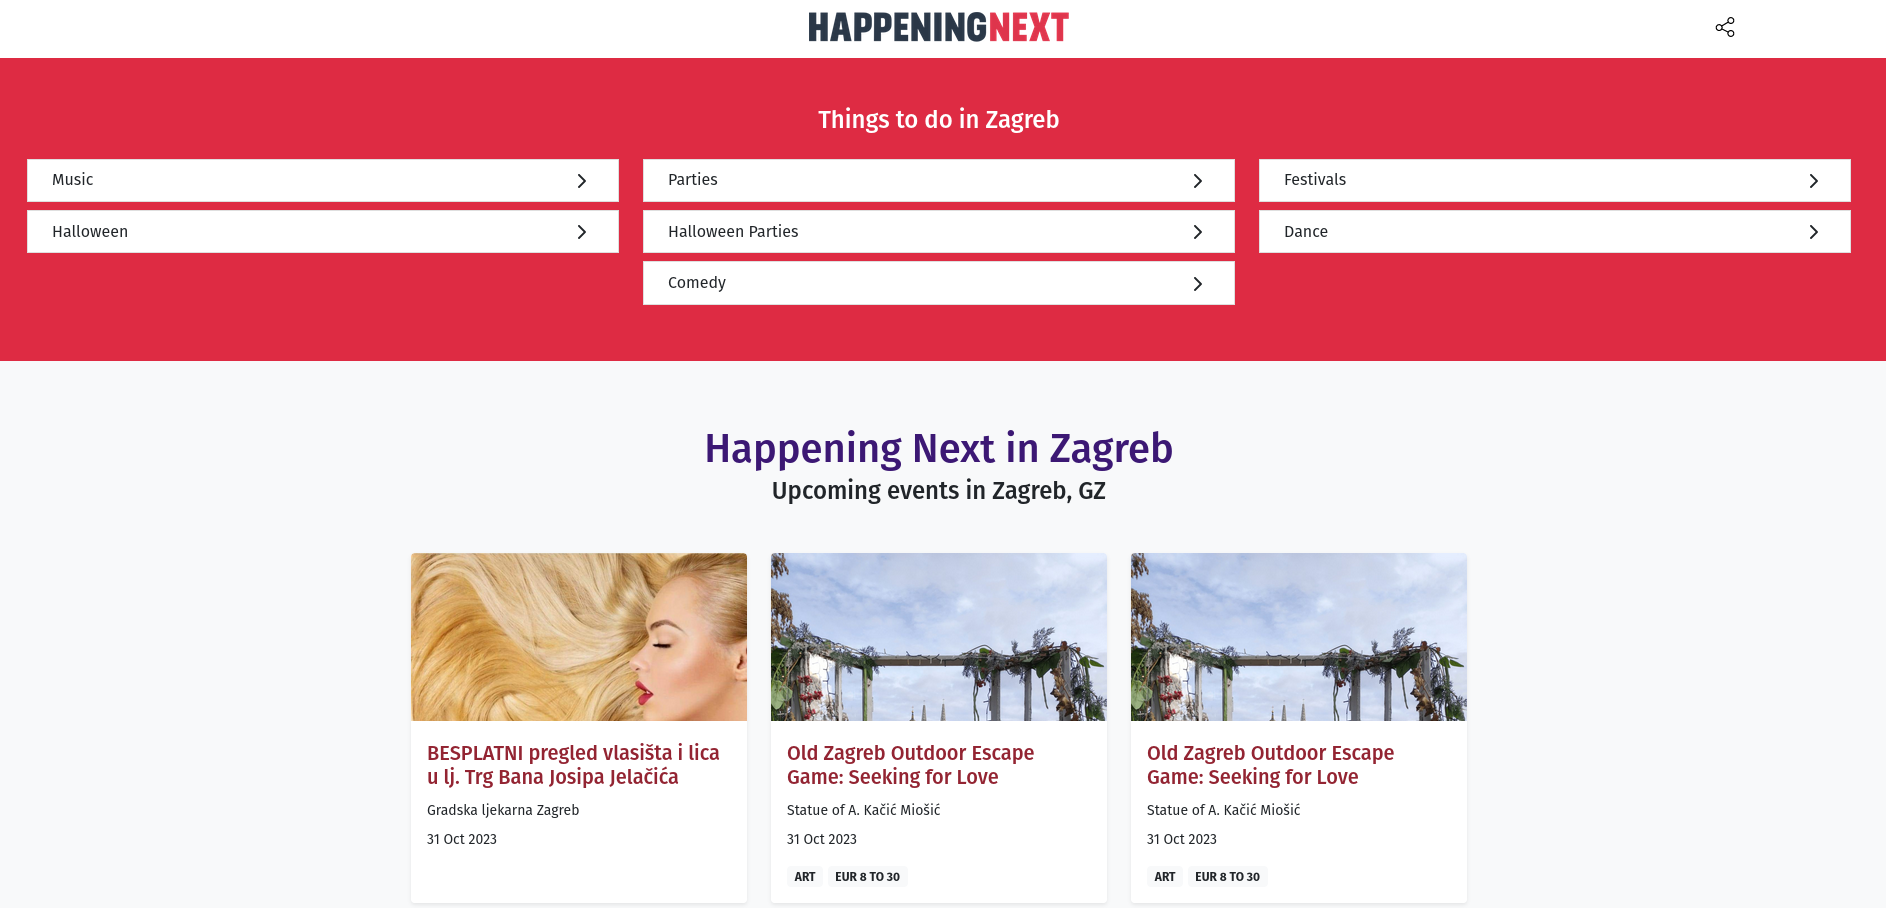
\includegraphics[scale=0.25]{slike/HappeningNext.png} 
		 	\centering
		 	\caption{HappeningNext}
		 	\label{fig:HappeningNext}
		 \end{figure}
		
		 \begin{figure}[H]
		 	
\includegraphics[scale=0.25]{slike/ConnectiNET.png} 
		 	\centering
		 	\caption{ConnectiNET}
		 	\label{fig:ConnectiNET}
		 \end{figure}

		ConnectiNET je trenutno dostupan samo na engleskom jeziku, ali je u budućnosti lako moguće dodati podršku za hrvatski jezik. Trenutno je dostupan samo u obliku web aplikacije, ali razvitak mobilne aplikacije bi doveo nove korisnike i omogućio bolju pristupačnost velikom dijelu postojećih korisnika. Također, u planu je dodati mogućnost prijave putem Facebooka i Google računa te integracija s tim platformama, poput mogućnosti dodavanja događaja u svoj Google kalendar ili direktno dijeljenje događaja na Facebook. Postoji još značajki koje bi u budućnosti unaprijedile sustav za koristnike, poput stranice s kartom na kojoj su prikazani događaji u blizini korisnika, mogućnost slanja poruka između korisnika koji se međusobno "prate", livestream-anje događaja i još mnogo toga. No, trenutno opseg aplikacije je već širok, s obzirom da svim korisnicima u određenim gradovima omogućuje međusobno povezivanje i pronalazak raznovrsnih zabavnih događaja u njihovoj blizini.

		Podržan je rad više korisnika u stvarnom vremenu te pristup iz javne mreže protokolom HTTPS. Sustav je jednostavan i brz za korištenje, te je u potpunosti siguran i pouzdan.

		\eject
		
		% \section{Primjeri u \LaTeX u}
		% 
		% \textit{Ovo potpoglavlje izbrisati.}\\
		% 
		% U nastavku se nalaze različiti primjeri kako koristiti osnovne funkcionalnosti \LaTeX a koje su potrebne za izradu dokumentacije. Za dodatnu pomoć obratiti se asistentu na projektu ili potražiti upute na sljedećim web sjedištima:
		% \begin{itemize}
		% 	\item Upute za izradu diplomskog rada u \LaTeX u - \url{https://www.fer.unizg.hr/_download/repository/LaTeX-upute.pdf}
		% 	\item \LaTeX\ projekt - \url{https://www.latex-project.org/help/}
		% 	\item StackExchange za Tex - \url{https://tex.stackexchange.com/}\\
		% 
		% \end{itemize} 	
		% 
		% 
		% 
		% \noindent \underbar{podcrtani tekst}, \textbf{podebljani tekst}, 	\textit{nagnuti tekst}\\
		% \noindent \normalsize primjer \large primjer \Large primjer \LARGE {primjer} \huge {primjer} \Huge primjer \normalsize
		% 		
		% \begin{packed_item}
		% 	
		% 	\item  primjer
		% 	\item  primjer
		% 	\item  primjer
		% 	\item[] \begin{packed_enum}
		% 		\item primjer
		% 		\item[] \begin{packed_enum}
		% 			\item[1.a] primjer
		% 			\item[b] primjer
		% 		\end{packed_enum}
		% 		\item primjer
		% 	\end{packed_enum}
		% 	
		% \end{packed_item}
		% 
		% \noindent primjer url-a: \url{https://www.fer.unizg.hr/predmet/proinz/projekt}
		% 
		% \noindent posebni znakovi: \# \$ \% \& \{ \} \_ 
		% $|$ $<$ $>$ 
		% \^{} 
		% \~{} 
		% $\backslash$ 
		% 
		% 
		% \begin{longtblr}[
		% 	label=none,
		% 	entry=none
		% 	]{
		% 		width = \textwidth,
		% 		colspec={|X[8,l]|X[8, l]|X[16, l]|}, 
		% 		rowhead = 1,
		% 	} %definicija širine tablice, širine stupaca, poravnanje i broja redaka naslova tablice
		% 	\hline \SetCell[c=3]{c}{\textbf{naslov unutar tablice}}	 \\ \hline[3pt]
		% 	\SetCell{LightGreen}IDKorisnik & INT	&  	Lorem ipsum dolor sit amet, consectetur adipiscing elit, sed do eiusmod  	\\ \hline
		% 	korisnickoIme	& VARCHAR &   	\\ \hline 
		% 	email & VARCHAR &   \\ \hline 
		% 	ime & VARCHAR	&  		\\ \hline 
		% 	\SetCell{LightBlue} primjer	& VARCHAR &   	\\ \hline 
		% \end{longtblr}
		% 
		% 
		% \begin{longtblr}[
		% 		caption = {Naslov s referencom izvan tablice},
		% 		entry = {Short Caption},
		% 	]{
		% 		width = \textwidth, 
		% 		colspec = {|X[8,l]|X[8,l]|X[16,l]|}, 
		% 		rowhead = 1,
		% 	}
		% 	\hline
		% 	\SetCell{LightGreen}IDKorisnik & INT	&  	Lorem ipsum dolor sit amet, consectetur adipiscing elit, sed do eiusmod  	\\ \hline
		% 	korisnickoIme	& VARCHAR &   	\\ \hline 
		% 	email & VARCHAR &   \\ \hline 
		% 	ime & VARCHAR	&  		\\ \hline 
		% 	\SetCell{LightBlue} primjer	& VARCHAR &   	\\ \hline 
		% \end{longtblr}
		% 
		% 
		% 
		% 
		% 
		% %unos slike
		% \begin{figure}[H]
		% 	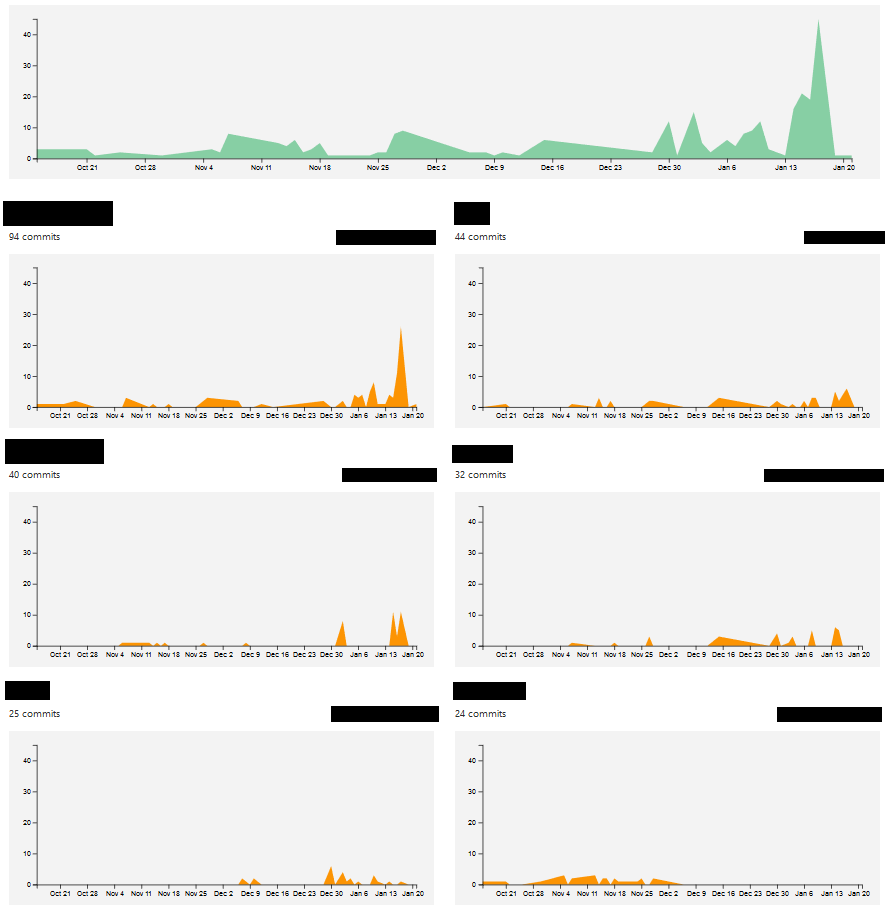
\includegraphics[scale=0.4]{slike/aktivnost.PNG} %veličina slike u odnosu na originalnu datoteku i pozicija slike
		% 	\centering
		% 	\caption{Primjer slike s potpisom}
		% 	\label{fig:promjene}
		% \end{figure}
		% 
		% \begin{figure}[H]
		% 	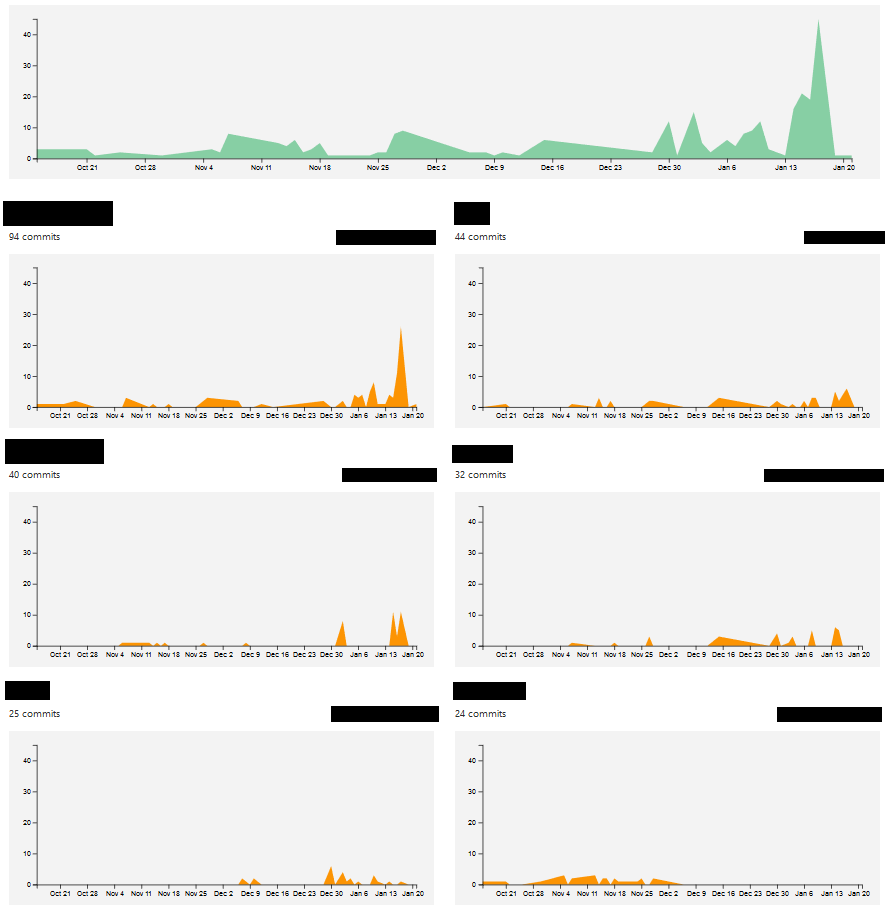
\includegraphics[width=\textwidth]{slike/aktivnost.PNG} %veličina u odnosu na širinu linije
		% 	\caption{Primjer slike s potpisom 2}
		% 	\label{fig:promjene2} %label mora biti drugaciji za svaku sliku
		% \end{figure}
		% 
		% Referenciranje slike \ref{fig:promjene2} u tekstu.
		% 
		% \eject
		
	